\section{UV Cutoff}
Even though the field is considered to be continuous, it ultimately arose from a lattice, so it can't vary on scales shorter than $a$. This means that the Fourier modes must vanish for suitably high momentum, i.e. $\phi(\boldsymbol{k})=0$ for $|\boldsymbol{k}|>\Lambda=\frac{\pi}{a}$. $\Lambda$ is called the ultraviolet cutoff.\\

\noindent Suppose that we only care about physics on long distance scales, $L$. Then we have no interest in the Fourier modes $\phi(\boldsymbol{k})$ with $k\gg\frac{1}{L}$. This suggests that we can write down a different theory, one that has a lower cut-off, $\Lambda'=\frac{\Lambda}{\zeta}$.\\

\noindent The Fourier modes can be written as $\phi(\boldsymbol{k})=\phi_-(\boldsymbol{k})+\phi_+(\boldsymbol{k})$, where $\phi_-(\boldsymbol{k})$ describe the long wavelength fluctuations and $\phi_+(\boldsymbol{k})$ describe the short wavelength fluctuations that we don't care about. $\phi_-(\boldsymbol{k})$ is non-vanishing for $k<\Lambda'$, whereas $\phi_+(\boldsymbol{k})$ is non-vanishing for $\Lambda'<k<\Lambda$. Then, the free energy is written in Fourier space which can be decomposed as,

$$F[\phi(\boldsymbol{k})]=F_0[\phi_-(\boldsymbol{k})]+F[\phi_+(\boldsymbol{k})]+F_I[\phi_-(\boldsymbol{k}),\phi_+(\boldsymbol{k})]$$. 

\noindent The third term mixes the short and long wavelength modes. The partition function becomes,

\begin{align*}
    \begin{split}
        Z&=\int\prod_{k<\Lambda'}d\phi_-(\boldsymbol{k})\,e^{-F_0[\phi_-(\boldsymbol{k})]}\int\prod_{\Lambda'<k<\Lambda}d\phi_+(\boldsymbol{k})\,e^{-F_0[\phi_+(\boldsymbol{k})]}e^{-F_I[\phi_-(\boldsymbol{k}),\phi_+(\boldsymbol{k})]}\\
        &=\int\mathcal{D}\phi_-\,e^{-F'[\phi_-]}
    \end{split}
\end{align*}

\noindent We cannot yet compare the original theory with the scaled theory. This is because the theory is defined by both the free energy and the UV cut-off, and the two theories have different cut-offs. This means that the original theory can describe things that the new theory cannot, namely momentum modes above the UV cut-off.\\

\noindent To remedy this, the momenta in the new theory is scaled as $\boldsymbol{k}'=\frac{\boldsymbol{k}}{\zeta}$. Now $\boldsymbol{k}'$ takes values up to $\Lambda$, as $\boldsymbol{k}$ did in the original theory. The counterpart of this scaling in real space is $\boldsymbol{x}'=\frac{\boldsymbol{x}}{\zeta}$. This implies we are observing the system in larger length scales. Finally, the fields are also scaled as $\phi'(\boldsymbol{x}')=\sqrt{\gamma'}\phi(\boldsymbol{x})$ to normalize the coefficient of the gradient term. The full scaled free energy takes the form,

$$F_\zeta[\phi']=\int d^dx\, \left[\frac{1}{2}(\nabla\phi')^2+\frac{1}{2}\mu^2(\zeta)\phi'\,^2+g(\zeta)\phi'\,^4\right]$$

\noindent The coupling constants `flow' as $\zeta$ increases. The original constants are evaluated at $\zeta=1$.

\section{Fixed Points}
If we keep on integrating out short distance degrees of freedom to generate a new theory again and again, there are essentially two possibilities - we could flow off to infinity, or we could converge towards a fixed point. These are points which are invariant under a RG transformation. Fixed points describe theories that have no characteristic scale. If the original theory had a correlation length scale $\xi$, then the renormalised theory has a length scale $\xi'=\frac{\xi}{\zeta}$. Fixed points must therefore have either $\xi=0$ or $\xi=\infty$.\\

\noindent In the disordered phase, with $T>T_c$, enacting an RG flow reduces the correlation length, which is equivalent to increasing the temperature. As shown in the picture below, the spins become more randomized.

\begin{center}
    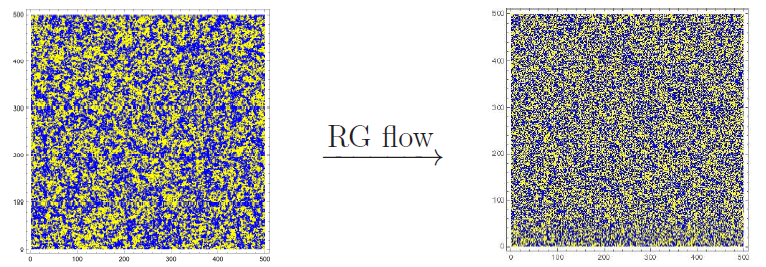
\includegraphics[scale=0.75]{disordered_rg}
\end{center}

\noindent Similarly, in the ordered phase also the RG flow reduces the correlation length. The end point at $\xi=0$ corresponds to the zero temperature limit. The spins become more aligned.

\begin{center}
    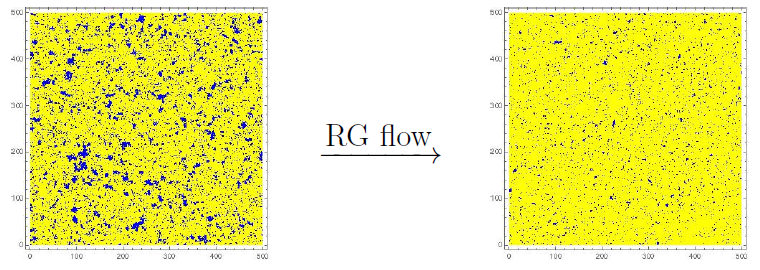
\includegraphics[scale=0.75]{ordered_rg}
\end{center}

\noindent Theories with $\xi=1$, occur at a critical point where the theory contains fluctuations on all length scales. Now, if we do an RG flow, the theory remains invariant. The configuration itself doesn't stay the same as it merely a representative configuration in the ensemble. However, as the fluctuations on small distance scales shrink away due to RG, they are replaced by fluctuations coming in from larger distance scales. In terms of visual configurations,

\begin{center}
    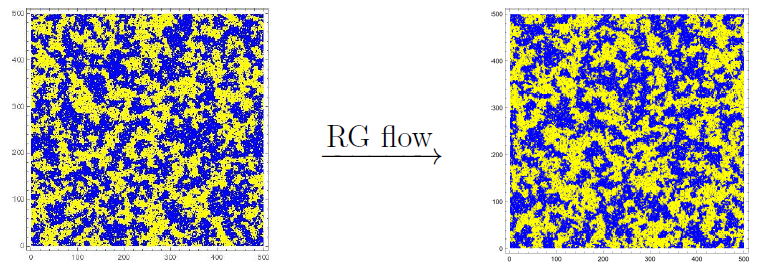
\includegraphics[scale=0.75]{critical_rg}
\end{center}

\noindent There are an infinite number of ways we can move away from the fixed point. If we move in some of these directions, the RG flow will take us back towards the fixed point. These deformations are called irrelevant because if we add any such terms to the free energy we will end up describing the same long-distance physics. In contrast, there will be some directions in which the RG flow will sweep us away from the fixed point. These deformations are called relevant because the long-distance physics will be different. Finally it's possible we simply end up on another fixed point. Such deformations are called marginal.

\section{Beta Functions}
Beta functions describe the flow of the coefficients of the field equation. After parameterizing the UV cutoff as $\Lambda'=\Lambda e^{-s}$, the beta functions are calculated by taking the derivative w.r.t. $s$.\\

\noindent For a free theory, there is no mixing between different coefficients. Any one does not induce a flow in the other. However, this no longer holds if the theory is interacting. Using Feynman rules, I have evaluated coefficients upto second order.

$$\mu^2(\zeta)=\zeta^2\left(\mu_0^2+12g_0\int_\frac{\Lambda}{\zeta}^\Lambda \frac{d^dq}{(2\pi)^d}\frac{1}{q^2+\mu_0^2}\right)$$
$$g(\zeta)=\zeta^{4-d}\left(g_0-36g_0^2\int_\frac{\Lambda}{\zeta}^\Lambda \frac{d^dq}{(2\pi)^d}\frac{1}{(q^2+\mu_0^2)^2}\right)$$\\

\noindent For small $s$, we have $\frac{d}{ds}\int_{\Lambda e^{-s}}^\Lambda dq\,f(q)\approx \Lambda f(\Lambda)$. Therefore, the beta functions become

$$\frac{d\mu^2}{ds}=2\mu^2+\frac{3g}{2\pi^2}\frac{\Lambda^4}{\Lambda^2+\mu^2}$$
$$\frac{dg}{ds}=-\frac{9g^2}{2\pi^2}\frac{\Lambda^4}{(\Lambda^2+\mu^2)^2}$$\\

\noindent The beta function for $\mu^2$ has two terms. The first term comes from the scaling procedures in RG, while the second comes from integrating out high momentum modes. Meanwhile, the beta function for $g$ only has a single term. There is no linear term in it because it was marginal under scaling, but it does receive a contribution when we integrate out the high momentum modes at second order.